\section{Processi di Supporto}


\subsection{Documentazione}
	
	\subsubsection{Scopo}
	\textcolor{red}{DA CORREGGERE: lo scopo della documentazione non dovrebbe essere scrivere documenti? lo scopo di questa sezione è descriverne le norme}
	Questo processo include e descrive le modalità di redazione e manutenzione dei documenti durante il ciclo di vita del prodotto software. Sono illustrate le norme, strumenti e convenzioni adottate per la scrittura di questi. Il tutto con l'obiettivo di consentire la stesura, senza ambiguità, di una documentazione valida, coerente e conforme a delle precise regole.
	
	\subsubsection{Procedure}
	\textcolor{red}{DA CORREGGERE: questo deve stare qui?}
	Il gruppo si è servito del linguaggio di markup {\LaTeX} per la stesura della documentazione.
	
		\paragraph{Approvazione dei documenti} \Spazio
		\textcolor{red}{CORRETTO: resposabile di progetto -> project manager}
		Ogni documento non formale in corrispondenza del completamento della sua stesura dovrà essere sottoposto al \textit{Project Manager}, che dovrà delegare ai \textit{Verificatori} il controllo del contenuto e della forma. Nel caso gli anzidetti \textit{Verificatori} rilevino degli errori, sarà loro compito notificarli al \textit{Project Manager}, che a sua volta affiderà il redattore del documento il compito di correggerli. Questo ciclo va eseguito fino a quando il documento non viene considerato completamente corretto dai  \textit{Verificatori}. In caso di assenso sulla correttezza e sulla qualità il documento può essere reputato un documento formale. In caso contrario spetta al \textit{Project Manager} comunicare le ragione per cui il documento non è stato giudicato corretto, esplicitando le modifiche da apportare.
		
	\subsubsection{Template}
	Per agevolare la redazione della documentazione è stato creato un template \LaTeX\text{ } contenente tutte le impostazioni stilistiche e grafiche citate in questo documento.
	
	\subsubsection{Struttura dei documenti}
	
		\paragraph{Prima pagina}\Spazio
		Ogni documento è caratterizzato da una prima pagina che contiene le seguenti informazioni sul documento:
		\begin{itemize}
			\item Logo del gruppo;
			\item Titolo del documento;
			\item Nome del gruppo;
			\item Nome del progetto;
			\item Versione del documento;
			\item Cognome e nome dei redattori del documento;
			\item Cognome e nome dei verificatori del documento;
			\item Cognome e nome del responsabile approvatore del documento;
			\item Destinazione d’uso del documento;
			\item Lista di distribuzione del documento;
			\item Una breve descrizione del documento.
		\end{itemize}
	
		\paragraph{Registro delle modifiche} \Spazio
		\label{registroModifiche}
		La seconda pagina di ogni documento contiene il registro delle modifiche del documento.
		Ogni riga del registro delle modifiche contiene:
		\begin{itemize}
			\item Un breve sommario delle modifiche svolte;
			\item Cognome e nome dell’autore;
			\item Ruolo dell’autore;
			\item Data della modifica;
			\item Versione del documento dopo la modifica.
		\end{itemize}
		La tabella contenente le modifiche è ordinata per data in ordine decrescente, affinchè la prima riga contenga la versione attuale del documento.
		
		\paragraph{Indici} \Spazio
		\textcolor{red}{DA CORREGGERE: (da correggere in altri documenti non qui)qui messo che ci sarà un indice  delle tabelle e delle figure: farlo presente agli altri. si usa il comando}
		In ogni documento, esclusi i verbali, è presente un indice delle sezioni, un indice delle figure e un indice delle tabelle. Nel caso non siano presenti figure o tabelle i rispettivi indici verranno omessi. La notazione numerica di ogni indice deve partire da 1 e le sottosezioni devono essere separate da un punto. Anche la notazione della sottosezione parte da 1.
		
		\paragraph{Formattazione generale delle pagine} \Spazio
		Il template prevede dei margini orizzontali e verticali che devono essere rispettati in ogni pagina. Ad esclusione della prima, tutte le pagine contengono un’intestazione ed un piè di pagina. 
			
			\subparagraph{Intestazione} \Spazio
			L’intestazione è così strutturata:
			\begin{itemize}
				\item Logo del gruppo posto a sinistra;
				\item Indirizzo di posta elettronica del gruppo posto a destra.
			\end{itemize}
			
			\subparagraph{Piè di pagina} \Spazio
			\textcolor{red}{da correggere: il nome del documento a questo punto deve avere anche la versione}
			Il piè di pagina è così strutturato:
			\begin{itemize}
				\item Nome e versione del documento corrente, posti a sinistra;
				\item Numerazione progressiva della pagina rispetto al totale posta a destra.
			\end{itemize}
		
		\paragraph{Note a piè di pagina} \Spazio
		In caso di presenza in una pagina interna di note da esplicare, esse vanno indicate nella pagina corrente, in basso a sinistra. Ogni nota deve riportare un numero e una	descrizione.
		
	\subsubsection{Versionamento}
	\label{versionamento}
	Tutti i documento, esclusi i verbali, devono essere versionati, affinchè si possa in ogni momento conoscerne la storia. Ogni versione di un documento deve essere appuntata nel Registro delle Modifiche. Si deve adottare il seguente formato per registrare ogni modifica: 
	\textbf{v{X}.{Y}.{Z}}
	dove:
	\begin{itemize}
		\item \textbf{X}
		\begin{itemize}
			\item Parte da 0;
			\item Viene incrementato dal \textit{Project Manager} in concomitanza con l'approvazione del documento;
			\item Arriva fino al numero di revisioni a cui è sottoposto il docuemnto.
		\end{itemize}
		
		\item \textbf{Y}
		\begin{itemize}
			\item Parte da 0;
			\item Viene incrementato dal Verificatore in concomitanza di ogni verifica;
			\item Quando X viene incrementato Y ritorna a 0.
		\end{itemize}
		
		\item \textbf{Z}
		\begin{itemize}
			\item Parte da 0;
			\item Viene incrementato dal \textit{Redattore} in concomitanza di ogni modifica;
			\item Quando Y viene incrementato Z	 ritorna a 0.
		\end{itemize}
		
	\end{itemize}
	
	\subsubsection{Norme tipografiche} 
	Per la redazione della documentazione bisogna attenersi alle seguenti norme.
		
		\paragraph{Stile del testo}
		\begin{itemize}
		\item \textbf{Grassetto:} il grassetto può essere utilizzato nei seguenti casi:
			\begin{itemize}
			\item \textbf{Elenchi puntati:} in questi casi può essere utilizzato il grassetto per evidenziare il concetto sviluppato nella continuazione del punto;
			\item \textbf{Altri casi:} per evidenziare particolari passaggi o parole chiave.
			\end{itemize}
		
		\item \textbf{Corsivo:} il corsivo deve essere utilizzato nei seguenti casi:
			\begin{itemize}
				\item \textbf{Citazioni:} quando si deve citare una frase questa va scritta in corsivo;
				\item \textbf{Abbreviazioni:} quando possibile si deve preferire una parola completa ad un’abbreviazione;
				\item \textbf{Nomi particolari:} il corsivo deve essere utilizzato quando si parla di figure particolari (es. \textit{Progettista});
				\item \textbf{Documenti:} il corsivo deve essere utilizzato quando si parla di documenti (es.\textit{Glossario});
				\item \textbf{Altri casi:} in altre situazione, il corsivo va utilizzato per mettere in rilievo passaggi o parole significativi, evidenziare riferimenti ai documenti interni o esterni.
			\end{itemize}
		
		\item \textbf{Maiuscolo:} l’utilizzo di parole completamente in maiuscolo è riservato solo agli acronimi.
		
		\end{itemize}
		
		\paragraph{Elenchi puntati} \Spazio
		Ogni punto dell’elenco deve terminare con un punto e virgola,tranne l’ultimo che deve terminare con un punto. La prima parola deve avere la lettera maiuscola, a meno di casi particolari (es. nome di un file);
		
		\paragraph{Formati comuni} \Spazio
		\label{formati}
		Per rappresentare le seguenti entità vanno usate le seguenti modalità:
		\begin{itemize}
			
			\item \textbf{Orari:}
			\textbf{HH:MM}
				\begin{itemize}
					\item \textbf{HH:} va da 0 a 23 e rappresenta l'ora;
					\item \textbf{MM:} va da 0 a 59 e rappresenta i minuti.
				\end{itemize}
			
			\item \textbf{Date:}
			\textbf{AAAA-MM-GG}
				\begin{itemize}
					\item \textbf{AAAA:} rappresenta l'anno;
					\item \textbf{MM:} rappresenta il mese;
					\item \textbf{GG:} rappresenta il giorno.
				\end{itemize}
			
			\item \textbf{Termini ricorrenti:}
			\begin{itemize}
				\item \textbf{Nomi proprio:} ogni nome proprio va scritto con il formalismo \textit{Nome Cognome};
				\item \textbf{Ruoli di progetto:} ogni ruolo va scritto con l'iniziale maiuscola e in corsivo;
				\item \textbf{Nomi dei documenti:} ogni documenti va scritto con l'iniziale maiuscola e in corsivo.
			\end{itemize}
			
		\end{itemize}
		
		\paragraph{Sigle} \Spazio
		\textcolor{red}{CORRETTO: tolte sigle che non usiamo}
		È previsto l’utilizzo delle seguenti sigle:
		\begin{itemize}
			\item AR: \textit{Analisi dei Requisiti};
			\item PP: \textit{Piano di Progetto};
			\item NP: \textit{Norme di Progetto};
			\item SF: \textit{Studio di Fattibilità};
			\item PQ: \textit{Piano di Qualifica};
			\item ST: \textit{Specifica Tecnica};
			\item MU: \textit{Manuale Utente};	
			\item MA: \textit{Manuale Amministratore}
			\item DP: \textit{Definizione di Prodotto};
			\item RR: Revisione dei requisiti;
			\item RP: Revisione di progettazione;
			\item RQ: Revisione di qualifica;
			\item RA: Revisione di accettazione;
		\end{itemize}
		
	\subsubsection{Elementi grafici}
		\paragraph{Tabelle}\Spazio
		Le tabelle presenti all'interno del documento devono essere centrate orizzontalmente nella pagina e devono presentare una didascalia sottostante avente un indice identificativo univoco incrementale per agevolarne il tracciamento, oltre che una breve descrizione del loro contenuto.\\
		Le tabelle del registro delle modifiche invece non hanno alcuna descrizione.
Qualora il redattore lo ritenesse necessario per aumentare la leggibilità è possibile anche l'uso di colori di sfondo scegliendone uno specifico per l'intestazione e due che verranno alternati per le righe sottostanti.

		\paragraph{Immagini}\Spazio
		Le immagini inserite nel documento sono nel formato PNG. Ognuna di esse deve essere accompagnata da una didascalia analoga a quella descritta per le tabelle. \\
		Ogni immagine deve inoltre essere centrata orizzontalmente mantenendo una separazione netta dai paragrafi che seguono e precedono, marcando quindi un distacco tra grafica e testo migliorando di conseguenza la leggibilità. \\
		I diagrammi UML vengono inseriti nei documenti sotto forma di immagine.
	\subsubsection{Classificazione dei documenti}
		\paragraph{Documenti informali}\Spazio
		Tutti i documenti sono informali dalla loro creazione fino all'approvazione da parte del \emph{Project Manager} ed in quanto tali sono considerati esclusivamente ad uso interno.
		\paragraph{Documenti formali}\Spazio
		Una volta avvenuta l'approvazione da parte del \emph{Project Manager} il documento viene ritenuto formale ed è quindi distribuibile all'esterno del gruppo.\\
		Per raggiungere tale stato inoltre, il documento deve aver già superato la fase di verifica e validazione. \\
Ogni modifica effettuata produrrà una nuova versione del documento da considerarsi informale e rimarrà tale fino ad una successiva approvazione da parte del \emph{Project Manager}.
		\paragraph{Verbali}\Spazio
		Dopo ogni incontro interno o esterno spetta al segretario verbalizzante redigere il documento. I verbali non sono soggetti a versionamento poiché non subiscono modifiche successive alla loro prima redazione. Deve avere un codice univoco identificativo con la seguente struttura: 
		\newline
		\centerline{[data]} 
		dove: 
    \begin{itemize} 
\item \textbf{data} è la data della riunione alla quale il verbale fa riferimento nel formato descritto in \ref{formati}. 
\end{itemize}
Dovrà presentare le seguenti informazioni nell'ordine in cui sono elencate:
\begin{itemize}
\item data, ora e luogo dell'incontro;
\item partecipanti presenti, assenti, il nome di chi presiede e quello del segretario verbalizzante;
\item l'ordine del giorno.
\end{itemize}
Tali informazioni devono essere contenute nel primo paragrafo \textit{Informazioni Generali}, che deve specificare anche gli argomenti trattati durante l'incontro.\\
Il secondo paragrafo \textit{Riassunto Incontro} deve esplicitare in dettaglio le decisioni prese o i problemi irrisolti.\\
Nel caso l'incontro abbia partecipanti esterni deve essere presente una sezione  \textit{Domande e Risposte} dove vengono riportate le domande poste, seguite dalle risposte date.
	\subsubsection{Strumenti}
		\paragraph{\LaTeX}\Spazio
		Per redigere i documenti viene utilizzato il linguaggio di markup \LaTeX. La possibilità di definire delle variabili all'interno dei fogli di stile consente di automatizzare l'aggiornamento di tutti i riferimenti presenti all'interno dei diversi documenti.\\
		Inoltre permette la creazione di documenti formali e divisi in sezioni molto velocemente, potendo separare il contenuto dalla formattazione tramite un file template separato e condiviso da tutti i documenti.\\
		Infine grazie all'elevato numero di librerie, permette di avere un'alta personalizzazione del documento.
		\paragraph{TexStudio}\Spazio
		L'editor scelto per sviluppare i documenti in \LaTeX\text{ } è TexStudio nella versione 2.12.6. 
		Lo strumento multipiattaforma integra un compilatore e un visualizzatore PDF, fornendo anche suggerimenti per completare i comandi \LaTeX.
		\newline\centerline{\href{http://www.texstudio.org/}{http://www.texstudio.org/}}
		\begin{figure}[H]
				\centering
				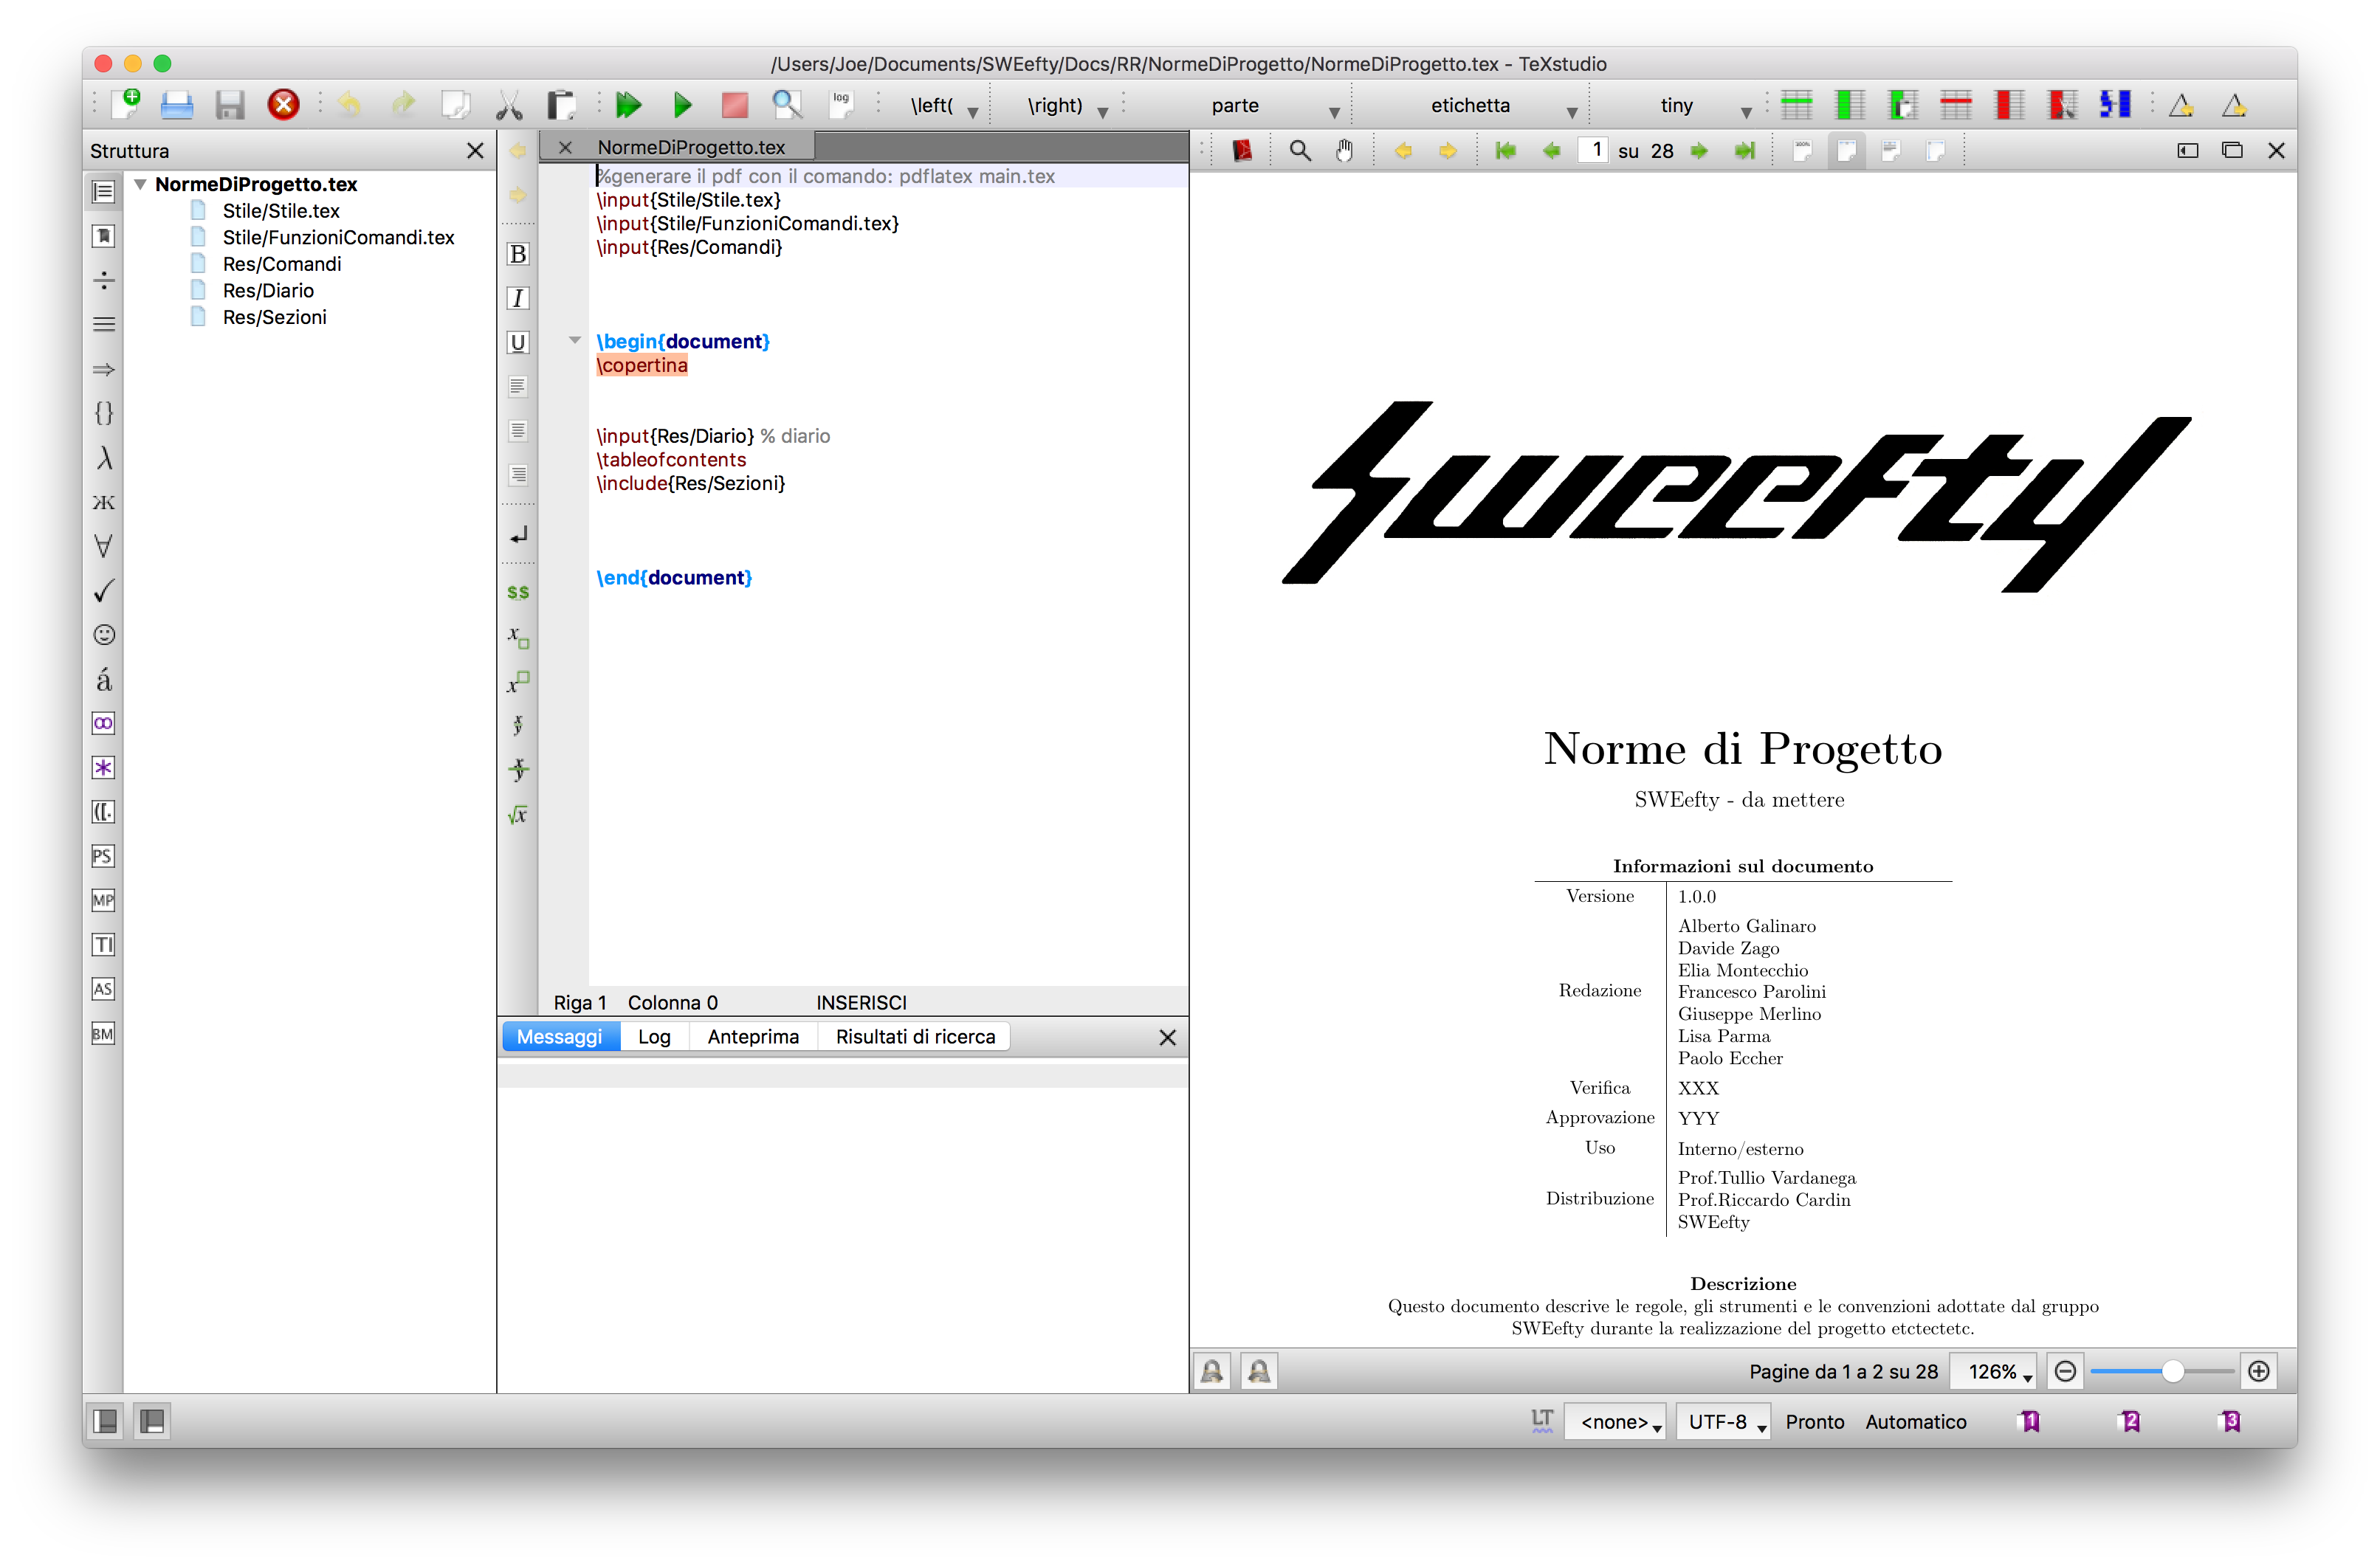
\includegraphics[width=1\textwidth]{Images/texstudio.png}
				\caption{TexStudio in versione desktop per Mac OSX}
			\end{figure}
			
\subsection{Verifica}

	\subsubsection{Scopo}
	La verifica accerta che l'esecuzione delle attività di processo attuate nel periodo in esame non abbia introdotto errori fornendo una prova oggettiva che dimostri di aver soddisfatto i requisiti definiti per i processi analizzati.
	Inoltre, si esamina la consistenza, completezza e correttezza del software prodotto e/o della documentazione redatta.
	\subsubsection{Attività}
		\paragraph{Analisi}
			\subparagraph{Analisi Statica} \Spazio
			L'analisi statica è una tecnica utilizzata per identificare errori all'interno di documenti e del codice sorgente, senza la necessità eseguirlo, è applicabile durante tutto il loro ciclo di vita in due diverse modalità:
			\begin{itemize}
				\item \textbf{Walkthrough}:
				consiste nel leggere il documento/codice cercando anomalie senza avere un'idea chiara di che tipo di errori possono essere trovati, è un'attività onerosa e non efficiente ma necessaria durante le prime fasi di progetto dove sarà la principale forma di verifica adottata, in quanto non è chiaro fin dall'inizio che tipo di errori si possono fare.
				Vista la sua scarsa efficacia normalmente viene effettuata da più persone.
				\item \textbf{Inspection}: 
				consiste nella lettura mirata del documento/codice per localizzare possibili errori specificati dalla lista di controllo. Ha un basso costo e diventa più efficace con l'esperienza e l'estensione della lista di controllo, per questo può essere effettuata da una persona sola.
			\end{itemize}
		    Ogni errore rilevato va discusso con l'autore allo scopo di concordare una modifica.
			\subparagraph{Analisi dinamica} \Spazio
			L'analisi dinamica è una forma di analisi del software che richiede l'esecuzione del codice sorgente. Viene effettuata tramite dei test che verificano il corretto funzionamento del prodotto, in caso di anomalie questi test aiutano ad identificare l'errore.
			I test devono essere ripetibili ovvero con lo stesso input e nello stesso ambiente devo essere in grado di ottenere sempre lo stesso output. Per ogni test sono quindi definiti i seguenti parametri:
			\textcolor{red}{DA CORRREGGERE: anche qui sotto da completare}
			\begin{itemize}
				\item \textbf{Ambiente}: sistema hardware e software sul quale si svolgerà il test;
				\item \textbf{Stato iniziale}: insieme dei valori assunti dalle variabili dinamiche prima dello svolgimento dei test;
				\item \textbf{Input}: i valori di ingresso specificati in ciascun caso di prova;
				\item \textbf{Output}: esito decidibile verificato rispetto a un comportamento atteso;
				\item \textbf{Istruzioni aggiuntive}: istruzioni su come va eseguito il test e su come vanno interpretati gli output.
			\end{itemize}
		\paragraph{Test}
			\subparagraph{Test di unità} \Spazio
			I test di unità verificano che le singole Unità di prodotto software funzionino correttamente, le unità non possono passare al test di integrazione se non passano questo test.
			Comunemente per i test di unità vengono utilizzati driver e stub che simulano il chiamante e un unità chiamata.
			\subparagraph{Test di integrazione} \Spazio
			I test di integrazione sono il passo successivo ai test di unità servono a verificare che due o più unità, precedentemente verificate, funzionino correttamente una volta combinate.
			Questo tipo di test verifica la corretta collaborazione tra le varie unità e aiuta a trovare eventuali errori non rilevati nei test precedenti.
			L'obbiettivo finale di questi test è arrivare a testare l'intero prodotto costituito accorpando tutte le singole unità.
			\subparagraph{Test di sistema} \Spazio
			I test di sistema validano il prodotto software ovvero si accertano che rispettino i requisiti concordati, vengono effettuati quando si ritiene che il prodotto abbia raggiunto una versione definitiva.
			\subparagraph{Test di regressione}	\Spazio
			I test di regressione devono essere fatti ogni volta che viene fatta una modifica a una componente software, consistono nel rifare i test di unità e integrazione necessari per accertarsi che tale modifica non causi errori nella componente in cui è stata fatta o in parti del software collegate.
			Un buon incapsulamento limita il numero di test da effettuare in questa fase.				
			\subparagraph{Test di accettazione} \Spazio
			Consiste nel collaudo del software in presenza del proponente, se questo test ha esito positivo il prodotto può essere rilasciato.
	\subsubsection{Strumenti}
			\paragraph{Verifica ortografica} \Spazio
			Viene utilizzato GNU Aspell, uno spell checker open source in grado di gestire più dizionari contemporaneamente che segnala gli errori all'interno di un documento mentre durante la scrittura viene utilizzato il controllo ortografico integrato in TeXstudio che segnala le parole errate sottolineandole in rosso.
			\paragraph{Analisi statica} \Spazio
			Per l'analisi statica del codice JavaScript viene utilizzato SonarJS, modulo di SonarQube in grado di rilevare bug e problemi di sicurezza, è inoltre disponibile su vari IDE come Eclipse e IntelliJ.
			\paragraph{Analisi dinamica} \Spazio
			Per l'analisi dinamica vengono utilizzati i seguenti software:
			\begin{itemize}
				\item  \textbf{Jest}: piattaforma per l'esecuzione di test su codice JavaScript, comodo per la sua semplicità di utilizzo.
				\item \textbf{Travis CI}: software usato per l' integrazione continua, una volta sincronizzato con la repository GitHub è in grado di eseguire automaticamente i test di integrazione, creati creati appositamente, su ogni commit in modo che si possa eseguire il comando push solo su codice che compila ed ha passato i test.
			\end{itemize}
			\paragraph{Metriche} \Spazio
			Per il calcolo delle metriche viene utilizzato SonarQube, software che permette di stabilire un grado di qualità che tutto il gruppo deve rispettare (come si vede in figura \ref{qualità}), inoltre permette di visualizzare grafici per controllare la qualità del progetto nel periodo di sviluppo (come si vede in figura \ref{graficobello}).
			\begin{figure}[h] 
				\centering 
				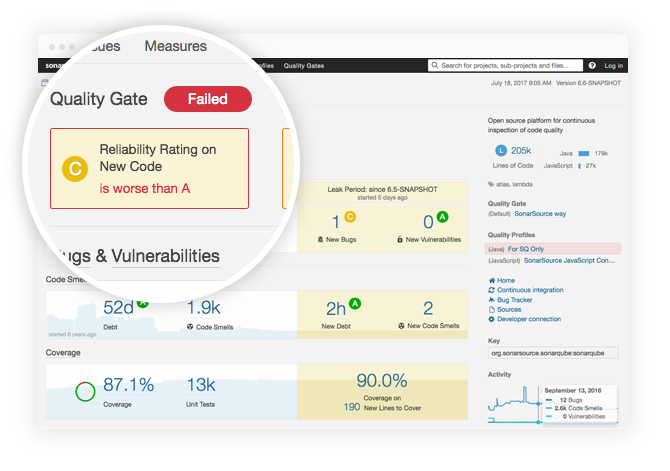
\includegraphics[width=0.9\textwidth]{images/enforce-quality-gate.png} 
				\caption{Dashboard con parametri di SonarQube}
				\label{qualità}
			\end{figure}
		    \begin{figure}[h]
		    	\centering 
		    	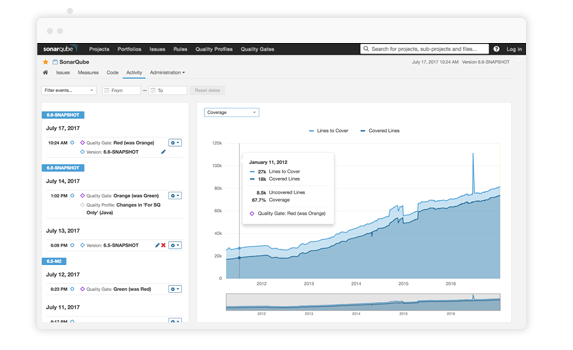
\includegraphics[width=0.9\textwidth]{images/project-history.png}
		    	\caption{Grafico prodotto da SonarQube}
		    	\label{graficobello} 
		    \end{figure}
			